\documentclass[a4paper, amsfonts, amssymb, amsmath, reprint, showkeys, nofootinbib, twoside]{revtex4-1}
\usepackage[spanish]{babel}
\usepackage[utf8]{inputenc}
\usepackage{float}
\usepackage[colorinlistoftodos, color=green!40, prependcaption]{todonotes}
\usepackage{amsthm}
\usepackage{mathtools}
\usepackage{physics}
\usepackage{xcolor}
\usepackage{graphicx}
\usepackage[left=23mm,right=13mm,top=35mm,columnsep=15pt]{geometry} 
\usepackage{adjustbox}
\usepackage{placeins}
\usepackage[T1]{fontenc}
\usepackage{lipsum}
\usepackage{csquotes}
\usepackage[normalem]{ulem}
\useunder{\uline}{\ul}{}
\usepackage[pdftex, pdftitle={Article}, pdfauthor={Author}]{hyperref} % For hyperlinks in the PDF
%\setlength{\marginparwidth}{2.5cm}

\begin{document}

%El título del experimento realizado es importante.
\title{Título del experimento}


\author{Carlos Devia}

%Si necesitan poner un segundo autor, deben eliminar los porcentajes (%) iniciales.
  
\author{Sergio Montoya}

\affiliation{Universidad de los Andes, Bogotá, Colombia.}

\date{\today} % Si lo dejan vacío no les saldrá fecha. La fecha que se muestra es del día en que se compila.

\begin{abstract}
% TODO Hacer el Abstract
\end{abstract}

\maketitle

\section{Objetivos}
\begin{enumerate}
  \item Estudiar la propagación de ondas mecánicas en la superficie del agua de una cubeta de ondas.
  \item Observar y analizar los fenómenos ondulatorios en el agua.
  \item Identificar frentes de onda y determinar las longitudes de onda en cada caso.
\end{enumerate}
\section{Analisis Cualitativo}
\begin{enumerate}
  \item \textbf{Enunciado:} Cuando tiene los dos perfiles de aluminio muy pegados, ¿qué efecto se puede ver?

        \textbf{Solución:} Difracción, ya que la propagación de una onda que se encuentra con un obstáculo que tiene una abertura, se podría pensar como la transmisión de la onda de un medio a otro

  \item \textbf{Enunciado:} ¿Qué efecto se está viendo con el video que se toma cuando se mueve la fuente puntual? ¿Qué pasaría si la fuente se mueve extremadamente rápido?

        \textbf{Solución:} Se está observando el Efecto Dooper, porque si la fuente que genera la onda, o el receptor se está moviendo, la frecuencia percibida por el receptor cambia respecto a si todos en el sistema se encuentran en reposo

  \item \textbf{Enunciado:} ¿Qué cambia con la propagación de la onda cuando se tiene refracción?

        \textbf{Solución:} Puede cambiar la dirección o incluso la velocidad de la onda, ya que cuando la onda que se propaga se encuentra con un obstáculo también entra a este, y por ende las propiedades del nuevo medio afectarán a la onda

  \item \textbf{Enunciado:} ¿Qué efecto se puede ver con las fuentes puntuales muy pegadas? ¿Hay algún otro caso que se vea similar a este?

        \textbf{Solución:} Interferencia, si dos ondas se encuentran y se combinan, de manera que la onda resultante es la suma física de las ondas. También podemos definir una interferencia constructiva si las dos ondas están en fase, o destructivas en el caso contrario, donde se encuentren en desfase
\end{enumerate}
\section{Analisis Cuantitativo}
Para cumplir con este requerimiento tenemos la fígura \ref{fig:tubito} con la cual podemos ver que la distancia de esta fuente es de 0.9
        \begin{figure}[h]
          \centering
          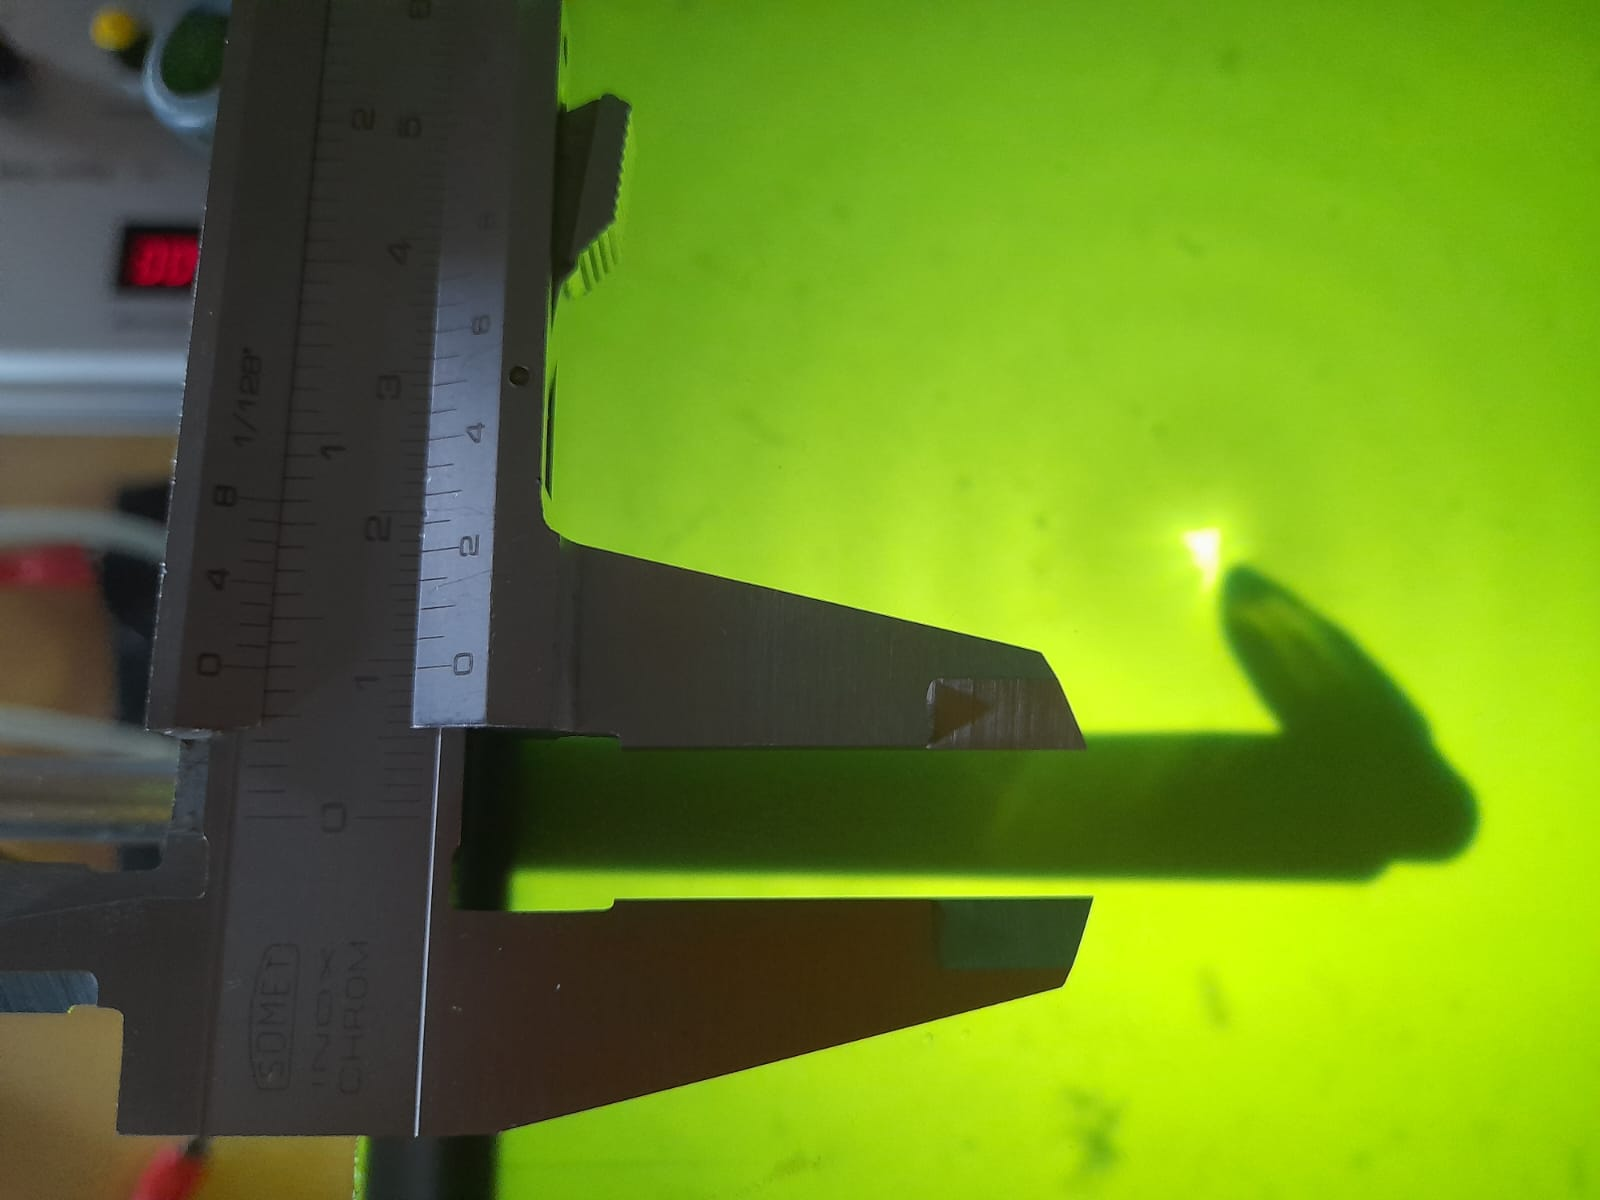
\includegraphics[scale=0.1]{tubito.jpeg}
          \caption{Grafica del tamaño del tubo desde el cual se dispersaban las ondas, Esta medida fue tomada de manera analoga y no tiene alteraciones digitales de manera consciente. El valor de esta distancia es entonces 0.9cm}\label{fig:tubito}
        \end{figure}
        Ahora bien, Vamos a utilizar las siguientes tres imagenes
        \begin{figure}[h]
          \centering
          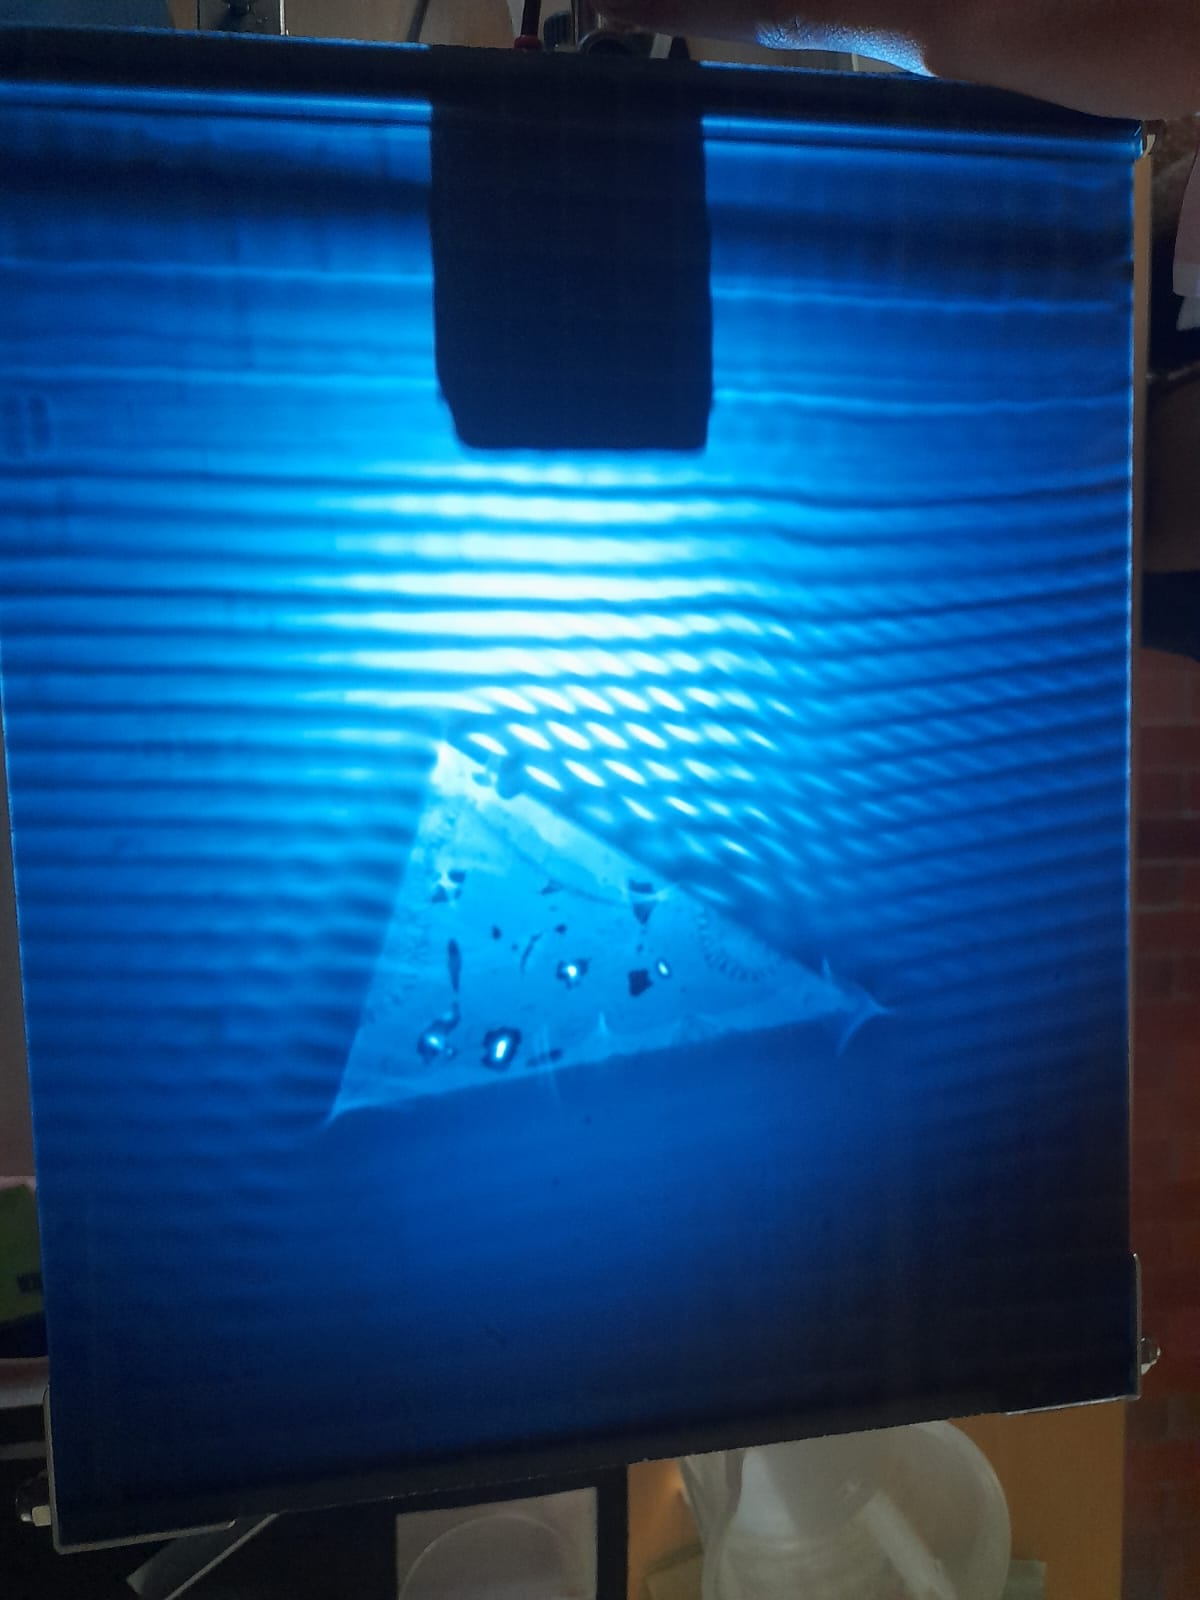
\includegraphics[scale=0.1]{Triangulo_Reflexion.jpeg}
          \caption{En esta figura se observa el fenomeno de reflexión y refracción. El primero, por que cuando el agua impacta con el triangulo este la refleja, se puede observar en la forma en la que la onda toma un angulo con respecto a la dirección original. El segundo efecto se ve en el triangulo pues la onda cambia de medio (en particular del agua al material del triangulo.)}\label{fig:Triangulo}
        \end{figure}
        \begin{figure}[h]
          \centering
          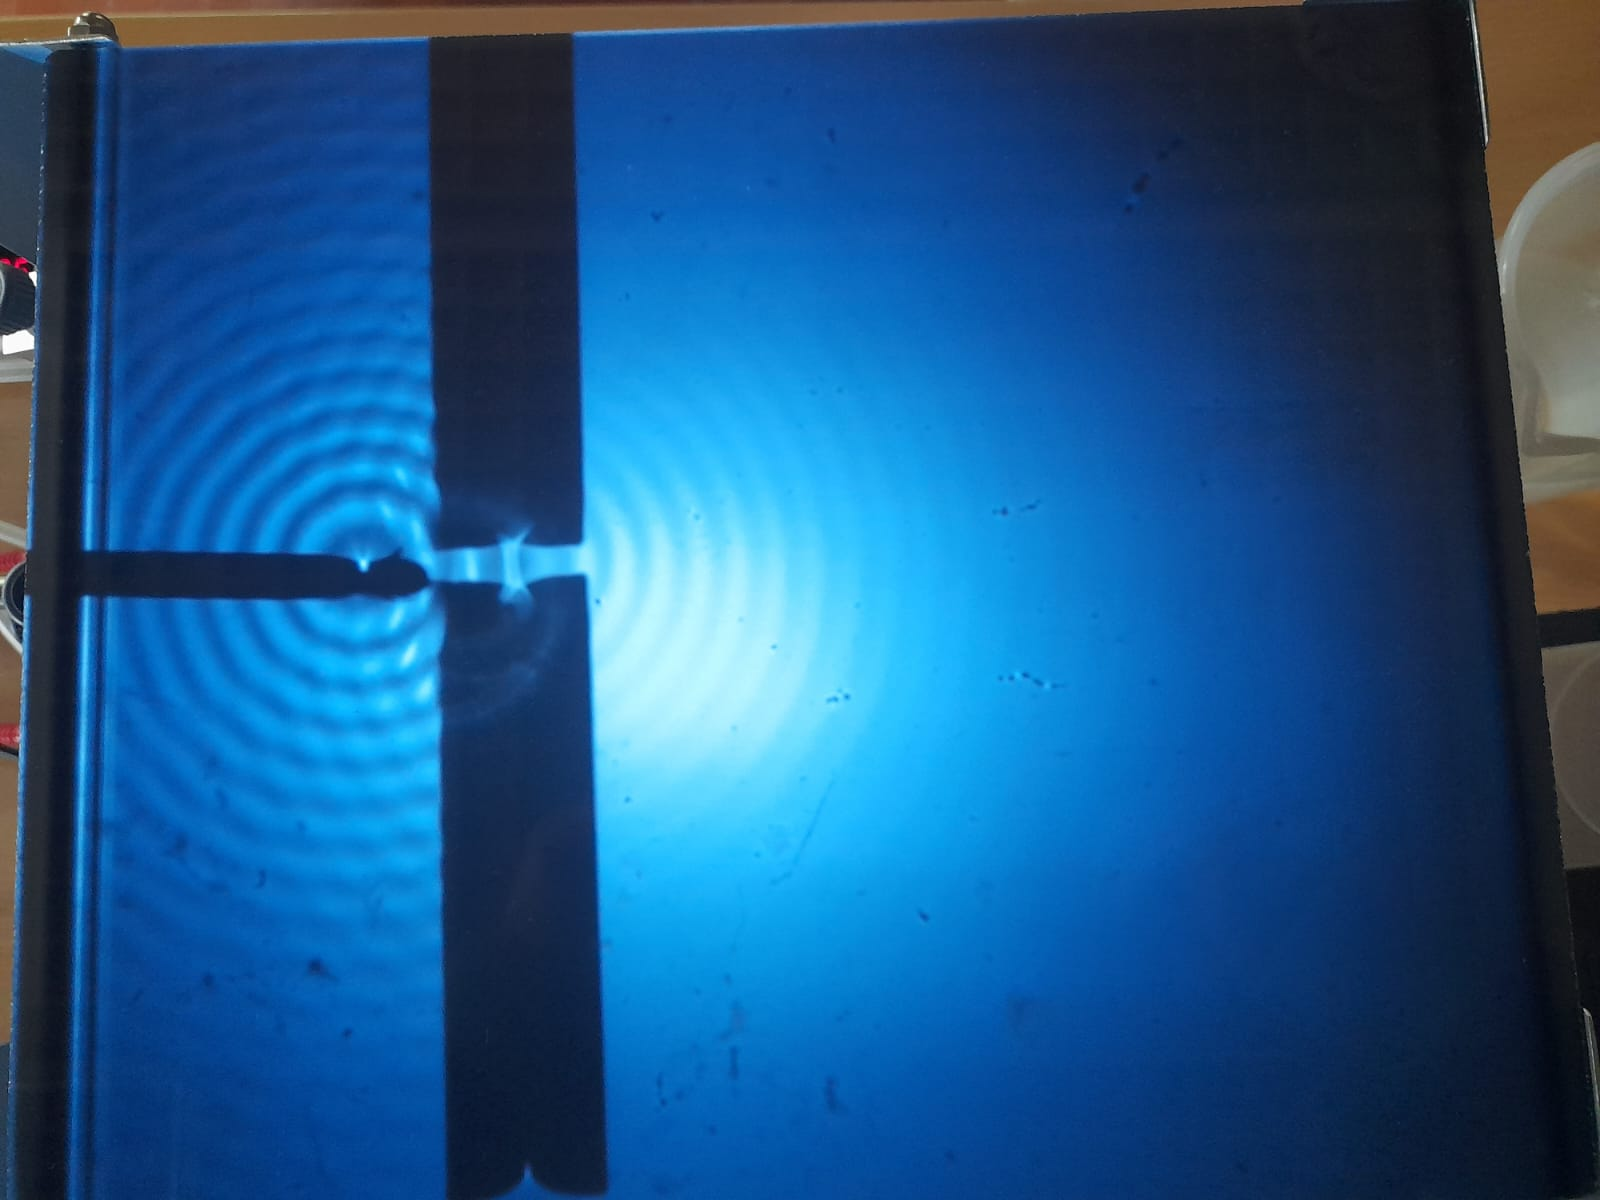
\includegraphics[scale=0.1]{Difraccion.jpeg}
          \caption{En esta figura se observa difracción. Esto pues la onda se encuentra con un obstaculo que no le permite continuar y por tanto la refleja pero ademas esta encuentra una via por la cual volverse puntual y seguir esparciendose.}\label{fig:Difraccion}
        \end{figure}
        \begin{figure}[h]
          \centering
          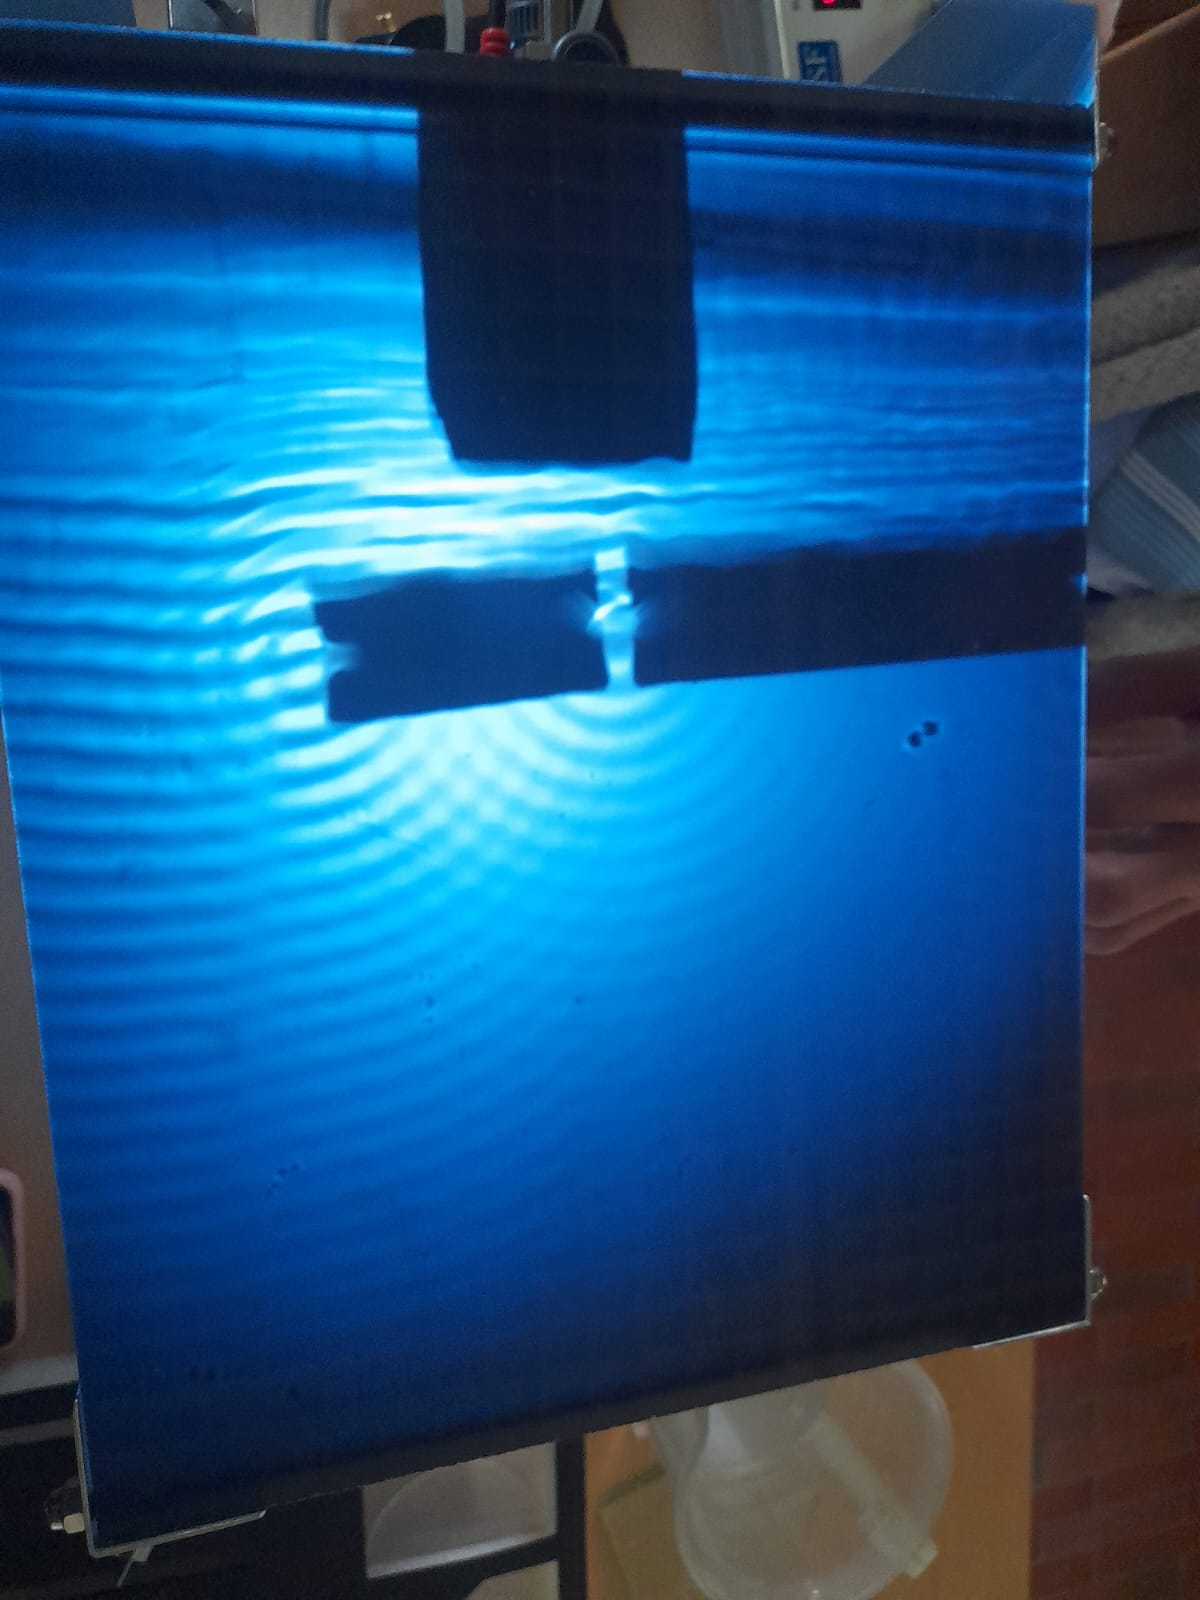
\includegraphics[scale=0.1]{Difraccion_2.jpeg}
          \caption{En esta imagen se observa Difracción e Interferencia. La primera, ocurre cuando la onda se dispersa unicamente por la apertura que se encuentra entre las barreras de metal. La segunda tiene ocasión una vez la onda se difracta pues interfiere con otro pedazo de si misma.}\label{fig:Difraccion2}
        \end{figure}

        Ahora bien, para la imagen \ref{fig:Triangulo} la separación de su longitud de onda en pixeles fue de 25 pixeles. La diferencia de pixeles de la imagen \ref{fig:Difraccion} es de 40 pixeles. Sin embargo, dado que tenemos la fuente como referencia podemos saber que esta mide 45 pixeles por lo cual la longitud de onda en este caso seria de 0.8 cm. Por ultimo, tenemos la imagen \ref{fig:Difraccion2} la cual tiene una longitud de onda en pixeles 50 pixeles.

        Por ultimo, para la comparación entre la ecuación $(6.3)$ y $(6.4)$ vamos a necesitar los siguientes datos
        \begin{enumerate}
          \item $g\approx 9.8 \frac{m}{s^{2}}$
          \item $h\approx 0.05 m$
          \item $\lambda \approx 0.008 m$
          \item $f = 60 Hz$
        \end{enumerate}
        Una vez tenemos todo esto lo unico que nos falta es realizar las operaciones pertinentes.
        \begin{align*}
          \nu &= \sqrt{9.8\cdot 0.005} = 0.49\\
          \nu &= 0.008\cdot60 = 0.48
        \end{align*}
\section{Conclusiónes}
Gracias al experimento pudimos ilustrar la propagación de ondas en dos dimensiones y observar los comportamientos de estas al ponerle diferentes objetos, cuando chocan, cuando atraviesan, como cambian de dirección y fenómeno como la difracción, interferencia, superposición de ondas y sobre todo el Efecto Doopler y entenderlo mejor. Además, se lograron identificar los frentes de onda para determinar las longitudes de estas en los casos deseados.
\end{document}
